%%%%%%%%%%%%%%%%%%%%%%%%%%%%%%%%%%%%%%%%%%%%%%%%%%%%%%%%%%%%%%%%%%%%%%%%%%%%%
%%%                                 Thermo                                  %%%
%%%%%%%%%%%%%%%%%%%%%%%%%%%%%%%%%%%%%%%%%%%%%%%%%%%%%%%%%%%%%%%%%%%%%%%%%%%%%
\subsubsection{Thermo}
\label{sec:uithermo}
A thermo shows the value of a data item in a graphical way.

\input{diagrams/ui_thermo_list}

\index{THERMO@\THERMO!ui\_manager thermo declaration}
\begin{tabularx}{\textwidth}{l|X}
THERMO Syntax       & description \\
\hline
\verb+IDENTIFIER+   & Thermo identifier (name). \\
\verb+ui xfer+      & Data item (see section \nameref{dia:uixfer} on page \pageref{dia:uixfer}). \\
\verb+scale factor+ & see section \nameref{sec:scale} on page \pageref{sec:scale}. \\
\end{tabularx}

\input{diagrams/ui_thermo_option}
\label{sec:uithermooption}

\index{RANGE@\RANGE!thermo option}
\index{OFFSET@\OFFSET!thermo option}
\index{COLOR@\COLOR!thermo option}
\index{COLOR\_SCALE@\COLORSCALE!thermo option}
\index{SCALE@\SCALE!thermo option!COLOR\_SCALE}
\index{ORIENTATION@\ORIENTATION!thermo option}
\index{SIZE@\SIZE!thermo option}
\index{FORMAT@\FORMAT!thermo option}
\index{LABEL@\LABEL!thermo option}
\index{UNIT@\UNIT!thermo option}
\index{ALARM\_LEVEL@\ALARMLEVEL!thermo option}
\index{ALARM\_COLOR@\ALARMCOLOR!thermo option}
\index{INVERTED@\INVERTED!thermo option}
\begin{tabularx}{\textwidth}{l|X}
thermo option            & description \\ 
\hline
\RANGE{} (min, max) & Thermo range from min to max. \newline
                    min, max can be constant (real\_value) or variable
                    (st\_data\_reference, see section \nameref{sec:stvariables}
                     on page \pageref{fig:st_data_reference}) \\
\OFFSET           & Offset added to the value before looking up the color in the \verb+ID_COLORSET+. \\
\COLOR            & Use colors defined in colorset (see section \nameref{sec:dpcolorset} page \pageref{sec:dpcolorset}) \\
\COLORSCALE       & The thermo is shown as a color scale. \newline
                    \SCALE: The colors (in the color scale) are interpolated. \\
\ORIENTATION      & Thermo orientation. \\
\SIZE{} (w, h)    & Width and height of the thermo in pixels. \\
\FORMAT           & Axis number format. \newline
                    ``10'' : width of the number \newline
                    %% ``10:2'' : width and decimals of the number \newline
                    ``10g'' : width of the number, change to scientific if number is too wide \\
\LABEL            & Thermo label. \\
\UNIT             & Thermo unit. \\
                  & \NONE{} : no label or unit. \\
                  & string : constant label or unit (see section \nameref{sec:string} on page \pageref{sec:string}). \\
                  & {\bfseries temp\_data\_reference} : variable label or unit (references a data item declared in the datapool,
                    see section \nameref{sec:tempdatareference} on page \pageref{sec:tempdatareference}). \\
\ALARMLEVEL       & Specify the alarm threshold. The part above this value is shown in \ALARMCOLOR. \\
\ALARMCOLOR       & Specify the alarm color. The part above \ALARMLEVEL{} is shown in this color. \\
\INVERTED         & Default is \TRUE. If set to \FALSE but max < min: use a different color. \\
\end{tabularx}
\vspace{0.5cm}

The following example shows the configuration of a thermo
and how it will be displayed by \INTENS{} (see page \pageref{fig:thermo})

\begin{boxedminipage}[t]{\linewidth}
\begin{alltt}
\UIMANAGER
  \THERMO
    speed_thermo {
      \RANGE ( speed_limit*0, speed_limit )
    , \COLOR = speed_color
    , \ORIENTATION = \VERTICAL
    , \SIZE ( 100, 200 )
    , \FORMAT = "4"
    , \LABEL = "Speed:"
    , \UNIT = \UNIT(speed)
    } ( 
      speed
    )
  ;
\END \UIMANAGER;
\end{alltt}
\end{boxedminipage}

\begin{figure}[h]\label{fig:thermo}
   \begin{center}
      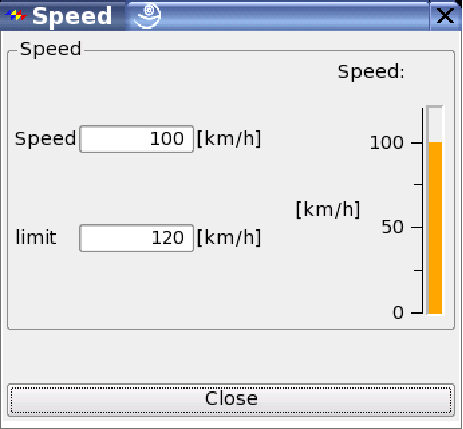
\includegraphics{grab_thermo}
   \end{center}
\caption{example of Thermo}
\end{figure}
